\newpage
\subsection{Beleuchtung}
\label{subsec:Beleuchtung}

Damit die Maschine optisch etwas hergibt, wurde entschieden die ganze Maschinerie mit LED-Streifen zu verzieren. Dazu ist einerseits das LED-Band von nöten und die geeignete Ansterung dazu. Für die Cocktailmaschine wurde festgelegt, dass der LED-Streifen die benötigten Wirderstände für die LED's schon aufgeklebt hat und die Ansteuerung folglich direkt über FET's geschehen kann. Der Aufbau ähnelt dann dem in Abbildung \ref{fig:LED1} gezeigten Schaltung. Der Streifen wäre Rot eingerahmt, die LED's und Widerstände befinden sich auf dem Band und die zu sehenden Fähnchen für R, G, B und W führen zum Mikrocontroller.

\begin{figure}[h!]
\center
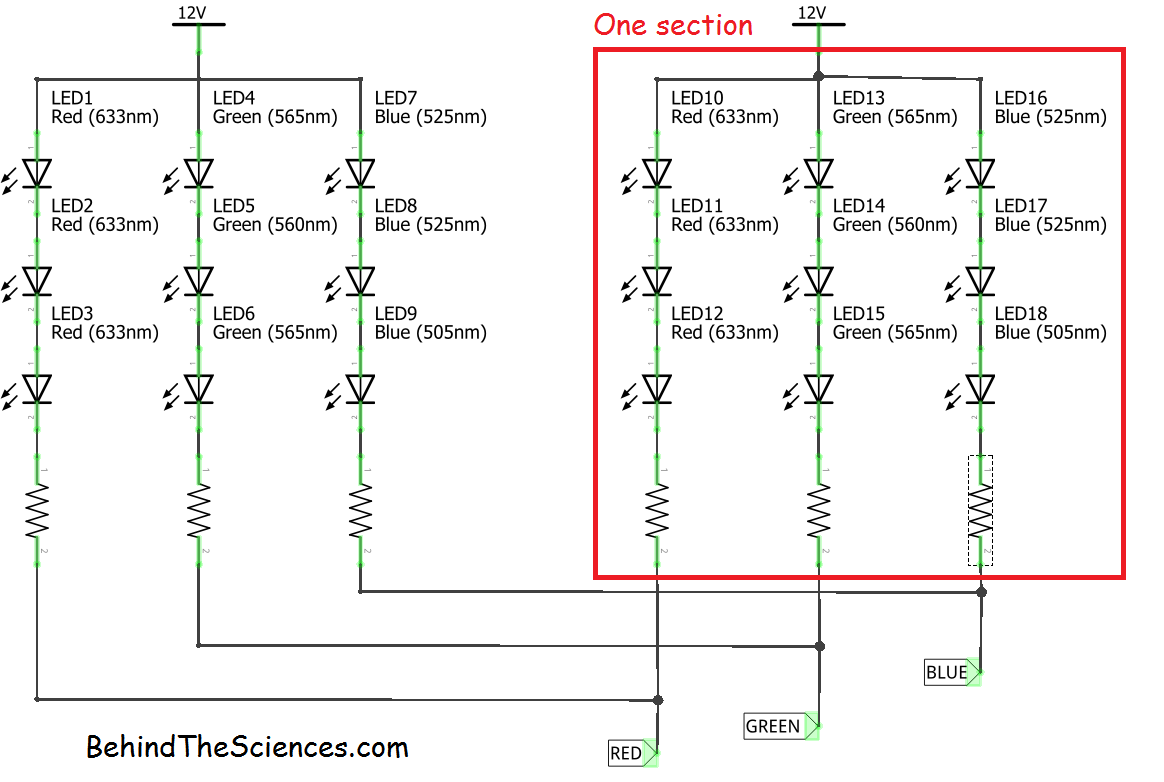
\includegraphics[width = \textwidth]{graphics/Schema_LED1}
\caption{Hallo}
\label{fig:LED1}
\end{figure}